\def\CTeXPreproc{Created by ctex v0.2.9, don't edit!}
%\documentclass{beamer}
\documentclass[%handout,
xcolor=pdftex]{beamer}
\mode<presentation> {
  \usetheme{Warsaw}
  \setbeamercovered{transparent}
}
\let\Tiny=\tiny
\usetheme{Singapore}
\usecolortheme{dolphin}
\usepackage{amsmath}
\usepackage{textcomp}
\usepackage{amssymb}
\usepackage{amsthm}
\usepackage{graphicx}
\usepackage{color}
\usepackage{lipsum}
\usepackage{hyperref}
\usepackage{multirow}
\usepackage{bm}
\DeclareMathSymbol{\Phi}{\mathalpha}{operators}{8}
%\setbeamertemplate{headline}{}
\setbeamertemplate{footline}[page number]
\newcommand\Fontvi{\fontsize{9pt}{8}\selectfont}
\newcommand\Fontvii{\fontsize{7pt}{8}\selectfont}
\newcommand{\backupbegin}{
   \newcounter{finalframe}
   \setcounter{finalframe}{\value{framenumber}}
}
\newcommand{\backupend}{
   \setcounter{framenumber}{\value{finalframe}}
}\newtheorem{proposition}{Proposition}
\title{Unit 19: Spectral Density for Causal ARMA Processes}
\author[STAT 5170: Applied Time Series, Unit 19]{Taylor R. Brown}
\institute{Department of Statistics, University of Virginia}
\date{Fall 2020}

\AtBeginSubsection[] {
  \begin{frame}<beamer>{Outline}
    \tableofcontents[currentsection,currentsubsection]
  \end{frame}
}



\begin{document}


\frame{\titlepage}

\begin{frame}
\frametitle{Readings for Unit 19}

Textbook chapter 4.2 (from page 176).

\end{frame}


\begin{frame}
\frametitle{Last Unit}
\begin{enumerate}
\item Spectral Density: Fourier Transformation of Autocovariance.
\item Properties of Spectral Density.
\end{enumerate}
\end{frame}

\begin{frame}
\frametitle{Motivation}

We generalize the spectral density for causal ARMA processes.

\end{frame}

\section{Spectral Density of Causal ARMA models}
\frame{\tableofcontents[currentsection]}

\begin{frame}
\frametitle{Causal ARMA Proccess}

A zero-mean causal ARMA process can be written as

$$
x_t = \sum_{j=0}^{\infty} \psi_j w_{t-j} = \psi(B)w_t.
$$

where $\psi(B) = \sum_{j=0}^{\infty} \psi_j B^j$. Therefore, the autocovariance function is

\begin{eqnarray*}
\gamma(h) &=& \mbox{E}(x_t x_{t+h}) \\
          &=& \mbox{E}(\sum_{j=0}^{\infty} \psi_j w_{t-j} \sum_{i=0}^{\infty} \psi_i w_{t+h-i}) \\
          &=& \sigma_w^2 \sum_{j=0}^{\infty} \psi_j \psi_{j+h}.
\end{eqnarray*}

\end{frame}

%\begin{frame}
%\frametitle{Autocovariance Generating Function}
%
%Define the autocovariance generating function as
%
%\begin{eqnarray} \label{eq:generate}
%g(B) &=& \sum_{h=-\infty}^{\infty} \gamma(h) B^h \\
%          &=& \nonumber \\
%          &=& \nonumber \\
%          &=& \nonumber \\
%          &=& \nonumber
%\end{eqnarray}
%
%\end{frame}

\begin{frame}
\frametitle{Spectral Density of Causal ARMA models}

Therefore the spectral density for a causal ARMA process can be expressed as

\begin{eqnarray} \label{eq:arma}
f(\omega) &=& \sum_{h=-\infty}^{\infty} \gamma(h) e^{-2 \pi i \omega h} \nonumber \\
          &=& \nonumber \\
          &=& \nonumber \\
          &=&
\end{eqnarray}

\end{frame}

\begin{frame}
\frametitle{Example: MA(q)}


\end{frame}

\begin{frame}
\frametitle{Example: AR(p)}


\end{frame}

\section{Rational Spectrum}
\frame{\tableofcontents[currentsection]}

\begin{frame}
\frametitle{Spectral Density of Causal ARMA models}


From (\ref{eq:arma}), we have

\begin{equation*} 
f(\omega) = \sigma_w^2 \left \lvert \frac{\theta(e^{-2 \pi i \omega})}{\phi(e^{-2 \pi i \omega})} \right \rvert ^2.
\end{equation*}

This is also called the \textbf{rational spectrum} of an ARMA(p,q).


\end{frame}

\begin{frame}
\frametitle{Zeroes and Poles}

Recall that every degree $p$ polynomial $a(z)$ can be factorized as

$$
a(z) = a_p(z-z_1)(z-z_2)\cdots(z-z_p)
$$

where $z_1, \cdots, z_p \in \mathbb{C}$ are the roots.

\end{frame}

\begin{frame}
\frametitle{Zeroes and Poles}

For the MA and AR polynomials,

$$
\theta(z) = \theta_q(z-z_1)(z-z_2)\cdots(z-z_q)
$$

and

$$
\phi(z) = \phi_p(z-p_1)(z-p_2)\cdots(z-p_p).
$$

$z_1,\cdots, z_q$ are called \textbf{zeroes}. $p_1,\cdots,p_p$ are called \textbf{poles}.

\end{frame}

\begin{frame}
\frametitle{Rational Spectrum}

Therefore, the rational spectrum as expressed in (\ref{eq:arma}) can be re-written as

\begin{eqnarray} \label{eq:poles}
f(\omega) &=& \sigma_w^2  \left\lvert \frac{\theta_q \prod_{j=1}^q \left( e^{-2 \pi i \omega} - z_j \right)}{\phi_p \prod_{j=1}^p \left( e^{-2 \pi i \omega} - p_j \right)} \right\rvert  ^2 \nonumber \\
          &=& \sigma_w^2 \frac{\theta_q^2 \prod_{j=1}^q \left\lvert e^{-2 \pi i \omega} - z_j \right\rvert ^2}{\phi_p^2 \prod_{j=1}^p \left\lvert e^{-2 \pi i \omega} - p_j \right\rvert ^2}.
\end{eqnarray}

\end{frame}


\begin{frame}
\frametitle{Examples: AR(1)}

Consider $\phi>0$.

\vspace{50mm}

\end{frame}

\begin{frame}
\frametitle{Examples: AR(1)}

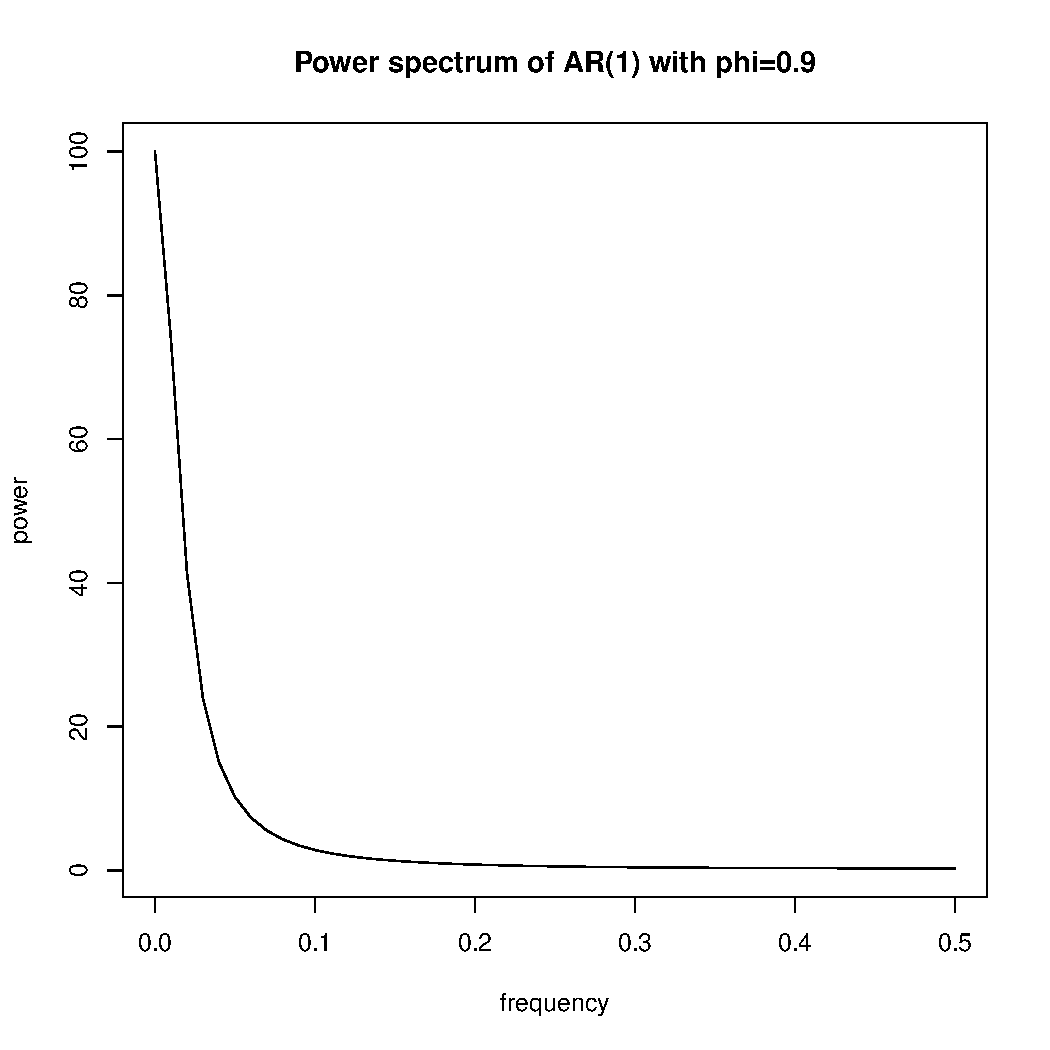
\includegraphics[width=100mm, height=80mm]{ar1_1power.pdf}

\end{frame}

%\begin{frame}
%\frametitle{Examples: AR(1)}

%Consider $\phi<0$.

%\vspace{50mm}

%\end{frame}

%\begin{frame}
%\frametitle{Examples: AR(1)}

%\includegraphics[width=100mm, height=80mm]{ar1_2power.pdf}

%\end{frame}

\begin{frame}
\frametitle{Examples: MA(1)}

Consider $\theta>0$.

\vspace{50mm}

\end{frame}

\begin{frame}
\frametitle{Examples: MA(1)}

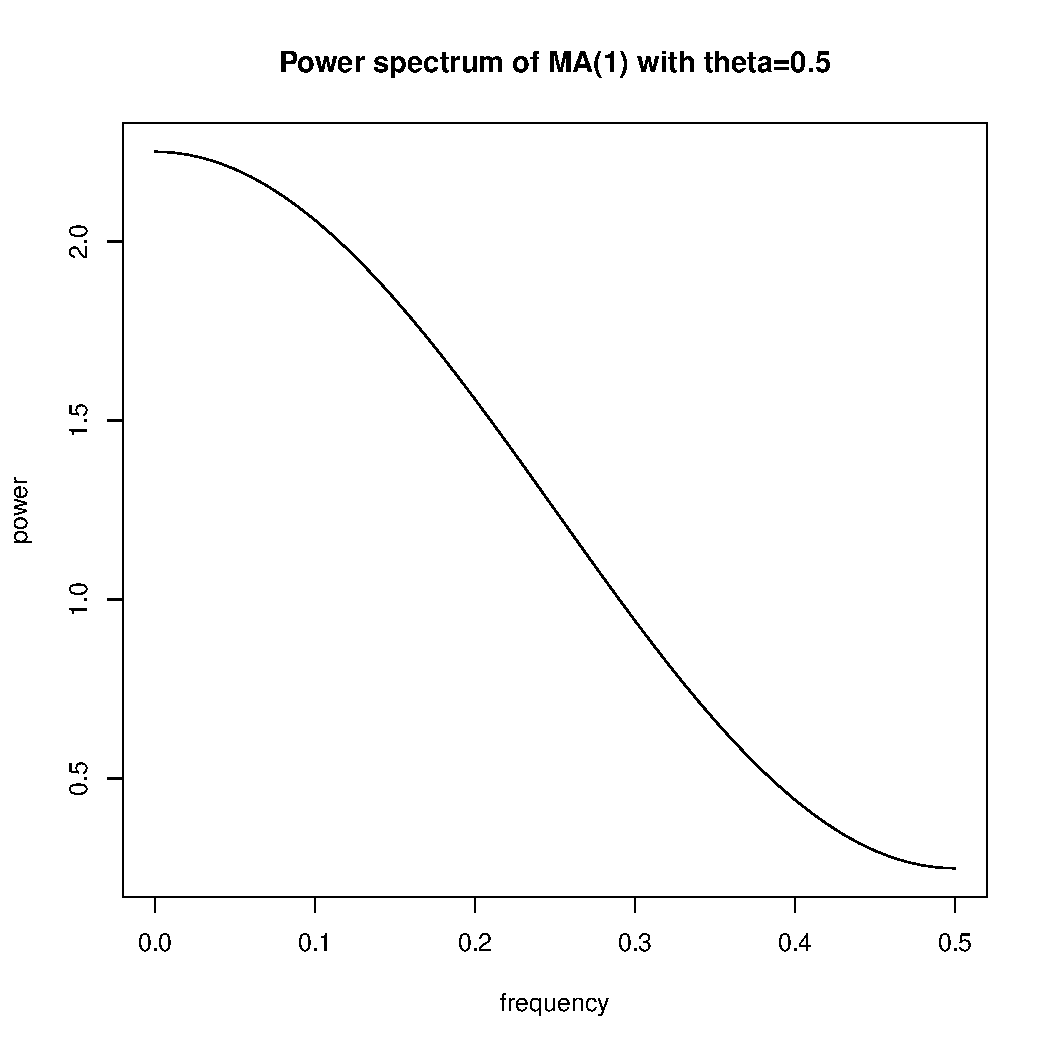
\includegraphics[width=100mm, height=80mm]{ma1_1power.pdf}

\end{frame}

%\begin{frame}
%\frametitle{Examples: MA(1)}

%Consider $\theta<0$.

%\vspace{50mm}

%\end{frame}

%\begin{frame}
%\frametitle{Examples: MA(1)}

%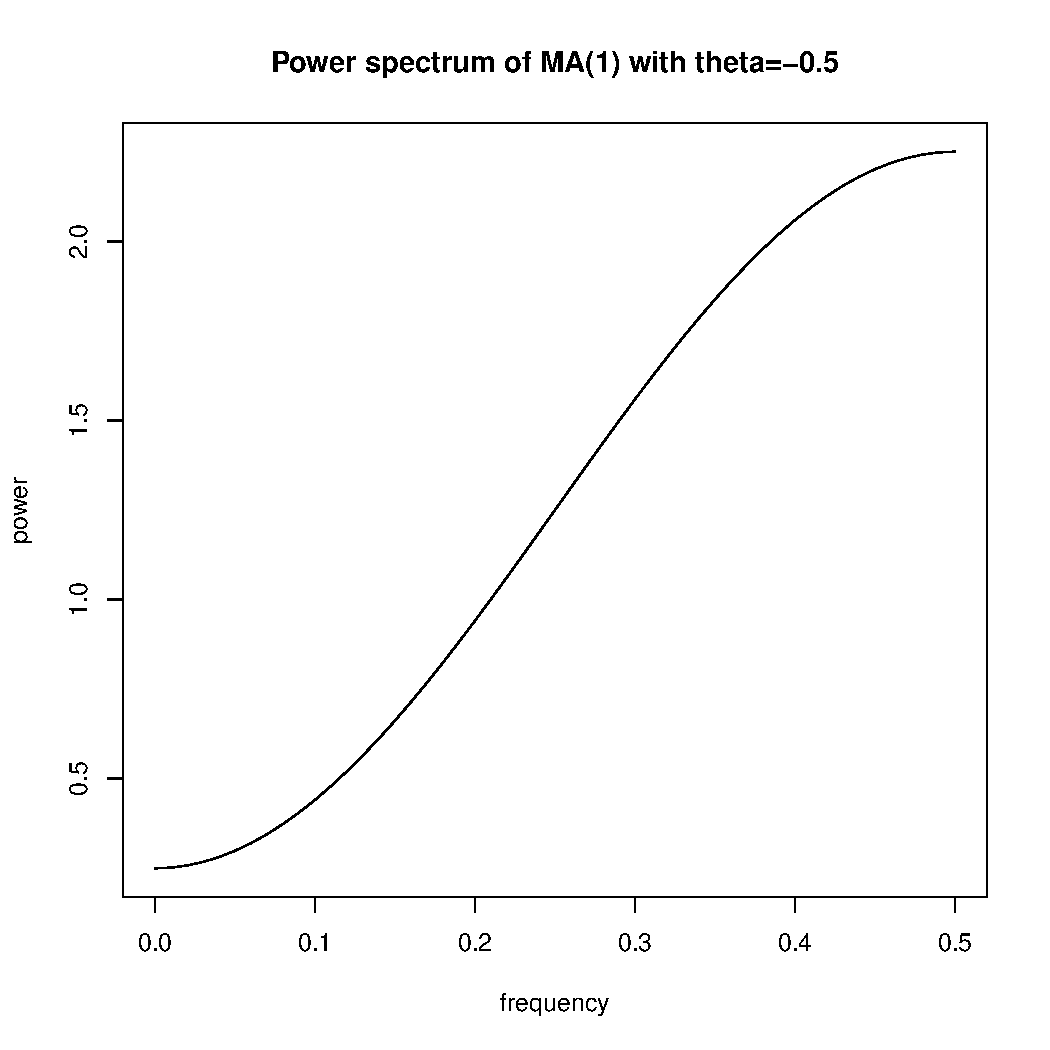
\includegraphics[width=100mm, height=80mm]{ma1_2power.pdf}

%\end{frame}

\begin{frame}
\frametitle{Examples: AR(2)}

Suppose we have the following AR(2) model: $x_t = x_{t-1} - 0.9 x_{t-2} + w_t$, where $\sigma_w^2 = 1$. The roots (poles) of the AR polynomial $\phi(z) = 0.9z^2 - z + 1$ are $p_1, p_2 = 0.555 \pm i0.8958$. Note that:

\vspace{40mm}

\end{frame}

\begin{frame}
\frametitle{Examples: AR(2)}

Using the representation (\ref{eq:poles}), the spectral density is

$$
f(\omega) = \frac{1}{\phi_2^2 \left \lvert e^{-2 \pi i \omega} - p_1 \right \rvert^2 \left \lvert e^{-2 \pi i \omega} - p_2 \right \rvert^2}.
$$

The peaks of the spectral density for this process occurs when $e^{-2 \pi i \omega}$ is near $1.054e^{-2 \pi i 0.16165}$.

\end{frame}

\begin{frame}
\frametitle{Examples: AR(2)}

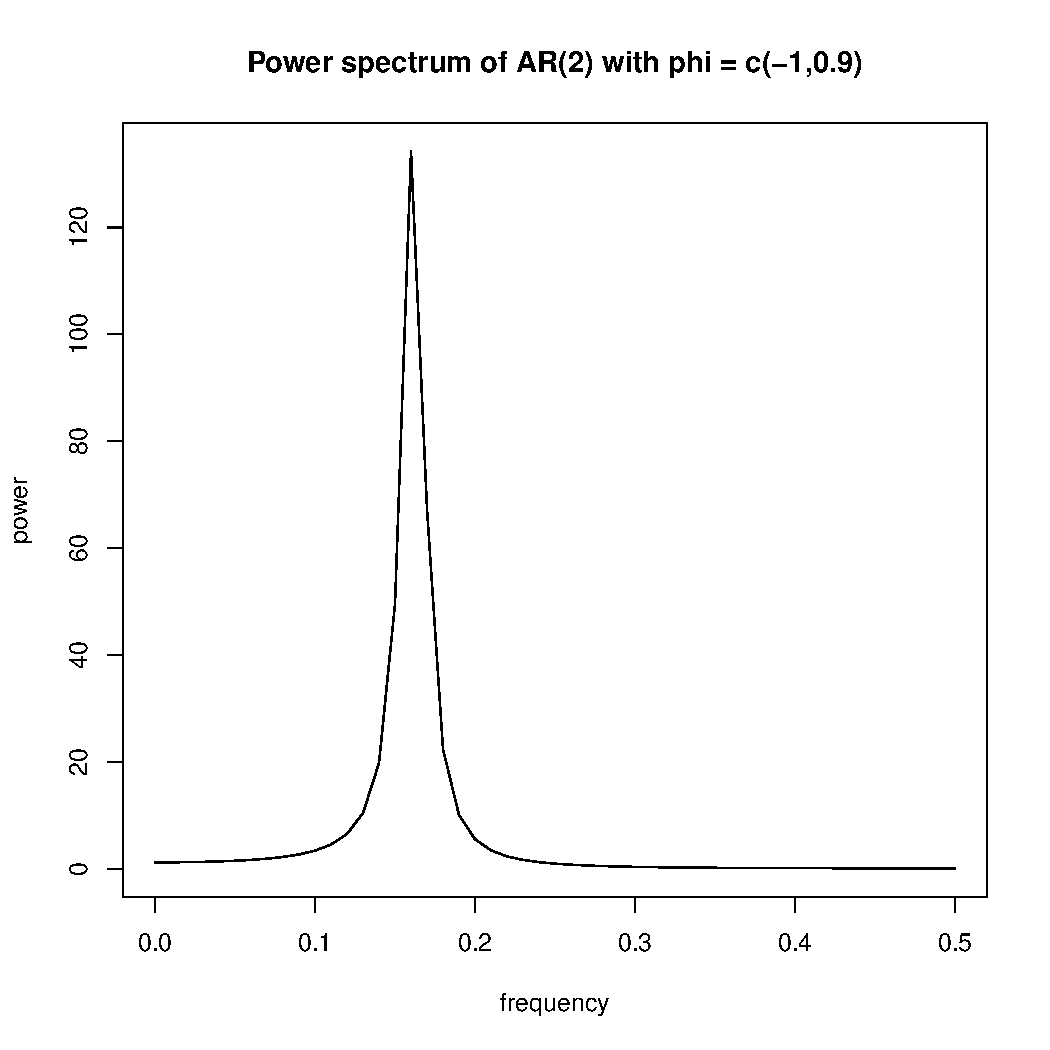
\includegraphics[width=100mm, height=80mm]{ar2power.pdf}

\end{frame}

\end{document} 